\documentclass[11pt,a4paper]{article}
\usepackage[margin=2.4cm]{geometry}
\usepackage{amsmath,amssymb,amsthm,graphicx,booktabs,microtype,xcolor}
\graphicspath{{../fig/}{fig/}}
\usepackage[colorlinks=true,linkcolor=blue!60!black,citecolor=blue!60!black]{hyperref}
\usepackage{enumitem}
\setlist{itemsep=3pt,parsep=0pt,topsep=4pt}
% generated by make_tables.py - do not edit
\newcommand{\Nstar}{1102}
\newcommand{\Sstar}{86}
\newcommand{\tstar}{3402}
\newcommand{\Ccoupling}{200}
\newcommand{\corebio}{81.5}
\newcommand{\nsubcore}{5}
\newcommand{\nhalo}{77}
\newcommand{\abscissa}{-1.000}
\newcommand{\deffsv}{2.17}
\newcommand{\deffeig}{5.67}
\newcommand{\nonnormality}{1.40}
\newcommand{\propcore}{5.8\times10^{-2}}
\newcommand{\propcoreNM}{2.4\times10^{-14}}
\newcommand{\prophaloNM}{4.2\times10^{-15}}
\newcommand{\rhoHalo}{+0.495}
\newcommand{\rhoMatched}{-0.002}
\newcommand{\rhoHaloPartial}{+0.067}
\newcommand{\rhoMatchedPartial}{+0.006}
\newcommand{\zHaloPartial}{+2.07}
\newcommand{\zMatchedPartial}{+0.06}
\newcommand{\rhoSelfHalo}{+0.491}
\newcommand{\rhoDecoupledHalo}{+0.088}
\newcommand{\silMatched}{+0.016}
\newcommand{\silZMatched}{-4.48}
\newcommand{\hopMeasured}{0.651}
\newcommand{\ariMatched}{-0.018}
\newcommand{\haloRho}{+0.69}
\newcommand{\haloRatio}{1.06}
\newcommand{\rankPred}{71}
\newcommand{\rankMeas}{62}
\newcommand{\coreFrac}{4}
\newcommand{\rhoJacHam}{+0.040}
\newcommand{\lamMax}{+3.09}
\newcommand{\lamRes}{-1.00}
\newcommand{\Nmin}{277}
\newcommand{\sigRatioAll}{7.1}
\newcommand{\sigRatioFix}{4.8}
\newcommand{\hopManifoldLo}{0.81}
\newcommand{\hopManifoldHi}{0.90}
\newcommand{\hopZmax}{-0.45}
\newcommand{\silManifoldLo}{0.05}
\newcommand{\silManifoldHi}{0.32}
\newcommand{\nregimes}{11}

\newcommand{\pk}{p_{\rm kill}}
\newcommand{\pmut}{p_{\rm mut}}
\newcommand{\poff}{p_{\rm off}}
\newcommand{\Hc}{H_{\rm crit}}
\newcommand{\Djac}{D_{\rm Jac}}
\newcommand{\R}[1]{\textcolor{blue!55!black}{[report, #1]}}

\title{\textbf{Supplementary Information: Analytical Derivations of the Survival Threshold, Halo Mutational Equilibrium, Dynamical Slaving Inversion, and Transition Mechanics}}
\author{Physics of Complex Networks --- Project 41\\Department of Physics and Astronomy ``G. Galilei'', University of Padua}
\date{\today}

\begin{document}
\maketitle

\tableofcontents

\newpage

\section{Microscopic Model Architecture and Ecological Constraints}
\label{sec:setup}

\subsection{Hypercube State Space and Quenched Asymmetric Couplings}

The Tangled Nature (TaNa) model~\cite{christensen2002tangled,anderson2004tangled,becker2014evolution,jensen2019tangled} describes coevolving individuals on a high-dimensional genomic sequence space. Genotypes are defined as binary bit strings $\mathbf{s} \in \{0,1\}^L$ of length $L = 20$, mapped to integers $a = \sum_{i=1}^L s_i 2^{i-1} \in [0, 2^{20}-1]$. Sequence space corresponds to the vertex set of a $20$-dimensional Boolean hypercube containing $2^{20} = 1{,}048{,}576$ vertices. The community configuration at generation $t$ is described by the occupancy vector $\mathbf{n}(t) = (n_1, \dots, n_{2^L})$, with total abundance $N(t) = \sum_a n_a(t)$ and diversity $S(t) = |\{a : n_a(t) > 0\}| \ll 2^L$.

Interspecies interactions are governed by a quenched coupling matrix $J(a,b)$ \R{Eq.~1} generated using bitwise XOR distance $a \oplus b$~\cite{rudyarthur-tnm}:
\begin{equation}
J(a,b) = \mathrm{mask}[a \oplus b] \cdot c[a \oplus b] \cdot g[b],
\label{eq:J_supp2}
\end{equation}
where $\mathrm{mask} \sim \mathrm{Bernoulli}(\theta = 0.25)$, $c \sim \mathcal{N}(0, 1)$, and $g \sim \mathcal{N}(0, C^2)$. Because $a \oplus a = 0$, diagonal self-interactions vanish identically ($J(a,a) = 0$). The commutative property $a \oplus b = b \oplus a$ guarantees that the underlying interaction topology is symmetric ($\mathrm{mask}[a \oplus b] = \mathrm{mask}[b \oplus a]$), while asymmetric donor weights $g[b] \neq g[a]$ generate coupling weight asymmetry ($J(a,b) \neq J(b,a)$). This weight asymmetry renders the resulting community Jacobian non-normal, generating non-orthogonal eigenmodes and non-reciprocal trophic interactions~\cite{trefethen2005spectra}.

\subsection{Fitness Function, Demographic Lifespan, and Generation Scaling}

The reproductive fitness $H_a(\mathbf{n})$ of an individual of genotype $a$ embedded within community $\mathbf{n}$ is given by \R{Eq.~2}:
\begin{equation}
H_a(\mathbf{n}) = \underbrace{\frac{1}{N} \sum_{b \neq a} J(a,b) n_b}_{H_I(a)\ \text{(cooperative gain)}} \;-\; \mu N \;-\; \nu N^2,
\label{eq:H_supp2}
\end{equation}
where $\mu = 0.10$ represents the linear resource carrying penalty, $\nu = 5 \times 10^{-6}$ provides quadratic damping, and abiotic fitness is set to zero ($\sigma = 0$). Offspring production follows the logistic transfer function:
\begin{equation}
\poff(H_a) = \frac{1}{1 + e^{-H_a}} \in (0,1).
\label{eq:poff_supp2}
\end{equation}

Microscopic dynamics advance through discrete elementary updates. In each step, an individual is chosen uniformly at random from the population to face mortality with probability $\pk = 0.20$, and an individual is chosen uniformly to attempt reproduction with probability $\poff(H_a)$, each offspring bit mutating independently with probability $\pmut = 0.01$. One generation is defined as $\tau = N / \pk$ elementary updates. Across one generation:
\begin{align}
\mathbb{E}[\#\text{death trials per individual}] &= \frac{N/\pk}{N} = \frac{1}{\pk} = 5, \\
\mathbb{E}[\#\text{deaths per individual}] &= \frac{1}{\pk} \cdot \pk = 1, \\
\mathbb{E}[\#\text{reproduction attempts per individual}] &= \frac{N/\pk}{N} = \frac{1}{\pk} = 5, \\
\mathbb{E}[\#\text{offspring produced per individual}] &= \frac{\poff(H_a)}{\pk}.
\end{align}
Thus, one generation corresponds exactly to the average lifespan of an undisturbed individual: the population turns over once on average per unit biological time.

\section{First-Principles Derivation of the Mean-Field Kinetic Equations}
\label{sec:meanfield}

\subsection{Master Equation and Microscopic Transition Rates}

Following the kinetic theory of individual-based coevolutionary models~\cite{cairoli2014forecasting,piovani2016linear}, let $P(\mathbf{n}, t)$ denote the probability distribution over community occupancy configurations $\mathbf{n} = (n_1, \dots, n_{2^L})^\top \in \mathbb{N}^{2^L}$ at continuous generation time $t$. Here, $\mathbf{e}_a$ denotes the standard canonical unit basis vector along the coordinate of genotype $a$, defined by $(\mathbf{e}_a)_b = \delta_{ab}$, such that $\mathbf{n} \pm \mathbf{e}_a = (n_1, \dots, n_a \pm 1, \dots, n_{2^L})^\top$ represents an elementary single-individual change in the community: an offspring birth incrementing genotype $a$ by $+1$ or a death decrementing genotype $a$ by $-1$, while leaving all other species abundances unchanged. The microscopic jump process is governed by the Master Equation:
\begin{equation}
\begin{split}
\frac{d P(\mathbf{n}, t)}{dt} = \sum_{a=1}^{2^L} \Big[ & W(\mathbf{n} + \mathbf{e}_a \to \mathbf{n}) P(\mathbf{n} + \mathbf{e}_a, t) + W(\mathbf{n} - \mathbf{e}_a \to \mathbf{n}) P(\mathbf{n} - \mathbf{e}_a, t) \\
& - \Big( W(\mathbf{n} \to \mathbf{n} - \mathbf{e}_a) + W(\mathbf{n} \to \mathbf{n} + \mathbf{e}_a) \Big) P(\mathbf{n}, t) \Big].
\end{split}
\label{eq:master_eq}
\end{equation}
In an elementary update step, the transition rate for a mortality decrement of species $a$ is:
\begin{equation}
W(\mathbf{n} \to \mathbf{n} - \mathbf{e}_a) = \frac{n_a}{N} \pk.
\end{equation}
The transition rate for an offspring increment of species $a$ produced by a parent of genotype $c$ is:
\begin{equation}
W(\mathbf{n} \to \mathbf{n} + \mathbf{e}_a) = \sum_{c=1}^{2^L} \frac{n_c}{N} \poff(H_c(\mathbf{n})) M(c \to a),
\end{equation}
where $M(c \to a) = \pmut^{\,h(c,a)} (1 - \pmut)^{L - h(c,a)}$ is the binomial mutation kernel on the hypercube with Hamming distance $h(c,a)$.

\subsection{Coarse-Graining}

To derive the continuous-time kinetic equations, we compute the first jump moment across one complete generation ($\tau = N / \pk$ elementary updates):
\begin{align}
\mathbb{E}[\Delta n_a] &= \tau \Big[ W(\mathbf{n} \to \mathbf{n} + \mathbf{e}_a) - W(\mathbf{n} \to \mathbf{n} - \mathbf{e}_a) \Big] \nonumber \\
&= \frac{N}{\pk} \left[ \sum_{c=1}^{2^L} \frac{n_c}{N} \poff(H_c(\mathbf{n})) M(c \to a) - \frac{n_a}{N} \pk \right] \nonumber \\
&= -n_a + \frac{1}{\pk} \sum_{c=1}^{2^L} n_c \, \poff(H_c(\mathbf{n})) \, M(c \to a).
\end{align}
Taking the continuous-time limit $\frac{dn_a}{dt} = \lim_{\Delta t \to 0} \frac{\mathbb{E}[\Delta n_a]}{\Delta t}$ yields the deterministic mean-field dynamics.

\subsection{Kinetic Rate Equation and Generation Scaling}

Thus, the mean-field kinetic rate equation governing genotype $a$ is \R{Eq.~5}:
\begin{equation}
\boxed{\;\frac{dn_a}{dt} = -n_a + \frac{1}{\pk} \sum_{c=1}^S n_c \, \poff(H_c(\mathbf{n})) \, M(c \to a).\;}
\label{eq:rate_supp2}
\end{equation}
The $-n_a$ term reflects natural mortality turning over the population at unit rate per generation; the summation term aggregates mutational recruitment from all reproducing parent lineages $c$.

\subsection{The Exact Autonomous Survival Threshold}
\label{sec:Hcrit}

In the low mutation regime ($p_{\text{mut}}\ll 1 \implies M(c \to a) \to \delta_{ca}$), Eq.~\eqref{eq:rate_supp2} reduces to isolated demographic growth:
\begin{equation}
\frac{dn_a}{dt} = n_a \left[ \frac{\poff(H_a)}{\pk} - 1 \right].
\end{equation}
A lineage can maintain positive or neutral demographic growth ($\frac{dn_a}{dt} \ge 0$) if and only if $\poff(H_a) \ge \pk$. Inverting the logistic function:
\begin{equation}
\frac{1}{1 + e^{-H_a}} \ge \pk \iff 1 + e^{-H_a} \le \frac{1}{\pk} \iff e^{-H_a} \le \frac{1 - \pk}{\pk} \iff H_a \ge \ln\left( \frac{\pk}{1 - \pk} \right).
\end{equation}
For $\pk = 0.20$, we obtain the exact \textit{autonomous survival threshold} \R{Eq.~3}:
\begin{equation}
\boxed{\;\Hc \equiv \ln\left( \frac{\pk}{1 - \pk} \right) = \ln(0.25) \approx -1.38629.\;}
\label{eq:Hcrit_supp2}
\end{equation}
Genotypes with $H_a < \Hc$ possess a reproduction probability strictly inferior to mortality ($\poff(H_a) < \pk$), driving them toward deterministic extinction unless continuously sustained by external mutational pumping.

\subsection{Global Carrying Capacity Balance at Stationarity}

At demographic stationarity ($\frac{dn_a}{dt} = 0$), summing Eq.~\eqref{eq:rate_supp2} over all species $a$ with $\sum_a M(c \to a) = 1$ gives:
\begin{equation}
\sum_{c=1}^S n_c^* \, \poff(H_c^*) = \pk N^* \iff \bar{p}_{\mathrm{off}} \equiv \frac{1}{N^*} \sum_{c=1}^S n_c^* \, \poff(H_c^*) = \pk = 0.20.
\label{eq:poff_balance_supp2}
\end{equation}
Because non-reproducing halo genotypes have $H_h \le -74.4$ ($\poff(H_h) \le 10^{-32}$), the sum is sustained entirely by the autonomous mutualistic core $\mathcal{C}$:
\begin{equation}
\sum_{c \in \mathcal{C}} n_c^* \, \poff(H_c^*) \approx \pk N^*.
\end{equation}
Since core species satisfy $H_c^* \approx \Hc$, the total population size $N^*$ is constrained by carrying capacity:
\begin{equation}
\frac{1}{N^*} \sum_{b \in \mathcal{C}} J(c,b) n_b^* - \mu N^* - \nu (N^*)^2 \approx \Hc \implies N^* \approx \frac{\bar{H}_{I,\mathrm{core}} - \Hc}{\mu}.
\label{eq:Nstar_scaling}
\end{equation}

\section{Analytical Mechanics of the Autonomous Survival Line}
\label{sec:line}

\subsection{Linear Carrying Capacity Target and Minimal Cooperative Gain}

Substituting the fitness definition Eq.~\eqref{eq:H_supp2} into the survival threshold Eq.~\eqref{eq:Hcrit_supp2} yields the condition for autonomous persistence:
\begin{equation}
\boxed{\;H_I(a) \equiv \frac{1}{N} \sum_{b \neq a} J(a,b) n_b \;\ge\; \mu N + \nu N^2 + \Hc\;.}
\label{eq:survival_line}
\end{equation}
The right-hand side is a macroscopic energetic threshold that depends on total population $N$, identical for every genotype. At our reference qESS plateau ($N = \Nstar$, $\mu = 0.10$, $\nu = 5 \times 10^{-6}$):
\begin{equation}
\mu N + \nu N^2 + \Hc = (0.10 \times 1102) + (5 \times 10^{-6} \times 1102^2) - 1.386 \approx 110.2 + 6.1 - 1.4 = 114.9 \approx 115.
\end{equation}
Every autonomously reproducing organism must secure a per-capita cooperative benefit $H_I(a) \ge 115$.

\subsection{Combinatorial Probability of Mutually Cooperative Cliques}
\label{sec:clique}

Because the quenched interaction matrix $J(a,b)$ has zero mean, a randomly assembled collection of genotypes yields an expected cooperative contribution $\mathbb{E}[H_I] = 0$. Diffuse, uncoordinated interactions cannot overcome the linear penalty $\mu N \approx 110$. Autonomous survival requires a tightly coordinated mutualistic clique $\mathcal{C}$ whose members share reciprocal positive couplings ($J(a,b) > 0$ and $J(b,a) > 0$).

Consider a candidate genotype $a$ attempting to establish mutual cooperative coexistence with an existing clique $\mathcal{C}$ of $k$ members. From Eq.~\eqref{eq:J_supp2}:
\begin{equation}
J(a,m) = \mathrm{mask}[a \oplus m] \cdot c[a \oplus m] \cdot g[m], \qquad J(m,a) = \mathrm{mask}[a \oplus m] \cdot c[a \oplus m] \cdot g[a].
\end{equation}
Because XOR is commutative, the topological factors $\mathrm{mask}[a \oplus m]$ and $c[a \oplus m]$ are shared between the forward and backward interactions. Both couplings are strictly positive if and only if:
\begin{equation}
\mathrm{mask}[a \oplus m] = 1, \quad \operatorname{sgn}(c[a \oplus m]) = \operatorname{sgn}(g[m]), \quad \text{and} \quad \operatorname{sgn}(c[a \oplus m]) = \operatorname{sgn}(g[a]).
\end{equation}
The latter two conditions force $\operatorname{sgn}(g[a]) = \operatorname{sgn}(g[m])$: every member of a mutually cooperative clique must share the identical sign of donor factor $g$. The candidate $a$ matches this donor sign with probability $1/2$. Conditioned on matching donor signs, each of the $k$ existing members independently requires:
\begin{itemize}
\item A topological connection: $\mathrm{mask}[a \oplus m] = 1$, which occurs with probability $\theta = 0.25$.
\item A compatible coupling sign: $\operatorname{sgn}(c[a \oplus m]) = \operatorname{sgn}(g[a])$, which occurs with probability $1/2$.
\end{itemize}
The joint probability that a candidate genotype forms reciprocal mutualistic links with all $k$ members of an existing clique is:
\begin{equation}
\boxed{\;P(a \text{ joins a } k\text{-clique}) = \frac{1}{2} \left( \frac{\theta}{2} \right)^k = \frac{1}{2} (0.125)^k.\;}
\label{eq:clique_prob}
\end{equation}
For $k = 2$, $P \approx 7.8 \times 10^{-3}$; for $k = 4$, $P \approx 1.2 \times 10^{-4}$; for $k = 6$, $P \approx 1.9 \times 10^{-6}$. Because a single negative coupling introduces fatal competitive drag (reducing fitness by $\sim 100$ units), viable mutualistic cliques are mathematically bounded to small sizes ($S_{\mathrm{core}} \in [2, 7]$ across all 12 parameter regimes in \R{Table~I}).

\subsection{Extreme-Value Scaling of Random Interaction Ensembles}

Could diffuse interactions among non-clique members clear the survival line through random Gaussian fluctuations? For a random set of $S$ interaction partners with donor scale $C = 200$, the variance of the uncoordinated cooperative sum is:
\begin{equation}
\operatorname{Var}\left( \frac{1}{N} \sum_{b=1}^S J(a,b) n_b \right) \approx \theta \, \sigma_c^2 \, \sigma_g^2 \sum_b \left( \frac{n_b}{N} \right)^2 = \theta \, C^2 \, \mathrm{IPR}_n.
\end{equation}
In a dispersed community with $\mathrm{IPR}_n \sim 1/S \sim 0.02$, the standard deviation is:
\begin{equation}
\sigma_{H_I} \approx \sqrt{0.25 \times 200^2 \times 0.02} \approx 14.1.
\end{equation}
Reaching the survival target $H_I \ge 115$ requires a fluctuation exceeding $115 / 14.1 \approx 8.15$ standard deviations:
\begin{equation}
P(H_I \ge 115)_{\mathrm{random}} \approx \frac{1}{\sqrt{2\pi}} \int_{8.15}^\infty e^{-u^2/2} du \approx 1.8 \times 10^{-16}.
\end{equation}
Even across the entire sequence space of $2^{20} \approx 10^6$ genotypes, the expected number of random configurations clearing the survival threshold is $\approx 10^{-10}$. Autonomous persistence through diffuse random interaction is statistically impossible.

\section{First-Principles Theory of the Stationary Mutational Halo}
\label{sec:halo}

\subsection{Non-Autonomous Halo Dynamics and Core Mutational Leakage}

For any halo genotype $h \notin \mathcal{C}$, autonomous reproduction is negligible: $H_h \le -74.4 \implies \poff(H_h) \le 10^{-32}$. The kinetic rate equation Eq.~\eqref{eq:rate_supp2} for a halo genotype simplifies to:
\begin{equation}
\frac{dn_h}{dt} \approx -n_h + \frac{1}{\pk} \sum_{c \in \mathcal{C}} n_c^* \, \poff(H_c^*) \, M(c \to h).
\end{equation}
Because mutation probability is small ($\pmut = 0.01$), the hypercube mutation kernel decays exponentially with Hamming distance $h(c,h)$:
\begin{align}
h(c,h) = 0 &: \quad (1 - \pmut)^L \approx 0.818, \nonumber \\
h(c,h) = 1 &: \quad \pmut (1 - \pmut)^{L-1} \approx 8.26 \times 10^{-3}, \nonumber \\
h(c,h) = 2 &: \quad \pmut^2 (1 - \pmut)^{L-2} \approx 8.34 \times 10^{-5}.
\end{align}
Transitions with $h \ge 2$ are suppressed by a factor $> 100$ relative to single-bit mutations. Mutational recruitment is dominated exclusively by 1-Hamming distance neighbors of the mutualistic core.

\subsection{Exact Parameter-Free Prediction of Stationary Halo Abundances}

Setting $\frac{dn_h}{dt} = 0$, stationary halo abundances satisfy:
\begin{equation}
n_h^* = \frac{1}{\pk} \sum_{c \in \mathcal{C}: h(c,h)=1} n_c^* \, \poff(H_c^*) \, M(c \to h).
\end{equation}
Because core mutualists maintain global demographic balance, their abundance-weighted offspring probability satisfies $\poff(H_c^*) \approx \pk$ (Eq.~\eqref{eq:poff_balance_supp2}). Substituting $\poff(H_c^*) / \pk \approx 1$ and $M(c \to h) = \pmut (1 - \pmut)^{L-1}$ yields \R{Eq.~9}:
\begin{equation}
\boxed{\;n_h^* \approx \pmut (1 - \pmut)^{L-1} \sum_{c \in \mathcal{C}: h(c,h)=1} n_c^*.\;}
\label{eq:halo_pred}
\end{equation}
Equation~\eqref{eq:halo_pred} contains \textbf{zero fitted parameters}: halo abundances are determined solely by the mutation rate $\pmut$, genome length $L$, and the abundances of 1-bit parent core mutualists.

\subsection{Empirical Validation Across Independent Parameter Regimes}

Testing Eq.~\eqref{eq:halo_pred} against empirical abundances across all $\nhalo$ non-reproducing halo genotypes at our checkpoint state yields:
\begin{itemize}
\item Spearman rank correlation: $\rho = \haloRho$.
\item Median ratio of observed to predicted abundance: $\operatorname{median}(n_h^{\mathrm{obs}} / n_h^{\mathrm{pred}}) = \haloRatio$.
\end{itemize}
As illustrated in \R{Fig.~2(b)}, the observed abundances follow the identity line over three orders of magnitude. The mutational halo is a statically slaved cloud of non-reproducing transients sustained entirely by mutational leakage from the reproducing core.

\section{Spectral Structure of the Community Jacobian and Breakdown of Slaving}
\label{sec:jacobian_spectrum}

\subsection{Analytical Community Jacobian and Block Structure}

Differentiating the deterministic mean-field abundance dynamics Eq.~\eqref{eq:rate_supp2} yields the closed-form community Jacobian matrix $K \in \mathbb{R}^{S \times S}$ evaluated at the stationary qESS microstate:
\begin{equation}
K_{ab} \equiv \frac{\partial \dot{n}_a}{\partial n_b} = -\delta_{ab} + \frac{1}{\pk} \left[ \poff(H_b) M(b \to a) + \sum_{c=1}^S n_c \, \poff'(H_c) \frac{\partial H_c}{\partial n_b} M(c \to a) \right],
\label{eq:K_explicit_supp2}
\end{equation}
where $M(c \to a) = \pmut^{D_H(c,a)} (1 - \pmut)^{L - D_H(c,a)}$ is the hypercube mutation kernel, $\poff'(H) = \poff(H)(1 - \poff(H))$, and the fitness derivative is:
\begin{equation}
\frac{\partial H_c}{\partial n_b} = \frac{J(c,b) - H_I(c)}{N} - \mu - 2\nu N.
\label{eq:dH_explicit_supp2}
\end{equation}
We partition the community into Core ($\mathcal{C}$, dimension $S_c = 4$) and Halo ($\mathcal{H} = \mathcal{S}_{\mathrm{sub}} \cup \mathcal{S}_{\mathrm{halo}}$, dimension $S_h = 82$). The Jacobian $K$ decomposes into $2 \times 2$ blocks:
\begin{equation}
K = \begin{pmatrix} K_{CC} & K_{CH} \\ K_{HC} & K_{HH} \end{pmatrix}.
\label{eq:K_blocks}
\end{equation}

\subsection{Algebraic Proof of Exact Unit Decay: The Rank-4 Perturbation Theorem}
\label{sec:rank4_proof}

At the reference plateau $t^* = \tstar$, the ecosystem partitions into $S_c = 4$ reproducing core mutualists concentrating $\corebio\%$ of total biomass ($898$ individuals) and $S_h = 82$ non-core genotypes comprising $5$ sub-core types ($n \in [6, 8]$) and $77$ halo genotypes ($n \le 5$, with $34$ singletons). 

Because every non-core genotype sits deeply within the sub-threshold lethal zone ($H_h \in [-133.6, -74.4] \ll \Hc = -1.386$), their reproductive probabilities and derivatives vanish to machine precision:
\begin{equation}
\poff(H_h) = \frac{1}{1 + e^{-H_h}} \le 5.03 \times 10^{-33} \approx 0, \qquad \poff'(H_h) \le 5.03 \times 10^{-33} \approx 0 \quad (\forall h \in \mathcal{H}).
\label{eq:poff_zero_halo}
\end{equation}
Substituting Eq.~\eqref{eq:poff_zero_halo} into the explicit Jacobian Eq.~\eqref{eq:K_explicit_supp2} reveals two fundamental mathematical simplifications:
\begin{enumerate}
    \item The direct offspring term $\poff(H_b) M(b \to a)$ vanishes identically for all non-core perturbation columns ($b \in \mathcal{H}$).
    \item In the recruitment sum $\sum_{c=1}^S$, all non-core parent contributions vanish identically because $\poff'(H_c) \approx 0$ for $c \in \mathcal{H}$.
\end{enumerate}
Consequently, the recruitment sum runs \emph{strictly over the $S_c = 4$ reproducing core mutualists}:
\begin{equation}
K_{ab} + \delta_{ab} = \frac{1}{\pk} \sum_{c=1}^{S_c=4} M(c \to a) \left[ \delta_{cb} \poff(H_c) + n_c \poff'(H_c) \frac{\partial H_c}{\partial n_b} \right] \equiv \sum_{c=1}^4 M_{ac} W_{cb}.
\label{eq:K_rank4_factorization}
\end{equation}
Equation~\eqref{eq:K_rank4_factorization} establishes an exact low-rank factorization for the \emph{shifted Jacobian matrix} $K + \mathbb{I}$ (where $\mathbb{I}$ denotes the $S \times S$ identity matrix). By ``shifted matrix'', we refer to the standard spectral shift $K - \lambda_0 \mathbb{I}$ evaluated at the halo mortality eigenvalue $\lambda_0 = -1$. Physically, the diagonal elements of the raw Jacobian $K$ contain an uncoupled death contribution $-\delta_{ab}$ arising directly from individual mortality ($-\pk \cdot n_a / \pk = -n_a$). The shifted matrix $K + \mathbb{I} = K - (-\mathbb{I})$ subtracts away this universal diagonal mortality background, isolating purely the net birth, recruitment, and mutational influx operator.

We express the system in terms of $K + \mathbb{I}$ because the unshifted Jacobian $K$ is full rank ($\operatorname{rank}(K) = 86$), whereas the isolated recruitment operator $K + \mathbb{I}$ factors into the product of an $(S \times 4)$ mutational basis matrix $\mathbf{M} \in \mathbb{R}^{S \times 4}$ and a $(4 \times S)$ sensitivity matrix $\mathbf{W} \in \mathbb{R}^{4 \times S}$:
\begin{equation}
K + \mathbb{I}_{S} = \mathbf{M}_{S \times 4} \, \mathbf{W}_{4 \times S} \implies \operatorname{rank}(K + \mathbb{I}) \le \min(4, S) = 4.
\label{eq:rank_bound}
\end{equation}
Singular value decomposition of $K + \mathbb{I}$ confirms this bound is exact: $\sigma_1 = 936.59$, $\sigma_2 = 167.00$, $\sigma_3 = 159.53$, $\sigma_4 = 82.80$, while $\sigma_5, \dots, \sigma_{86} \le 9.06 \times 10^{-14} \approx 0$. 

By the Rank-Nullity Theorem, the nullspace dimension of $K + \mathbb{I}$ is:
\begin{equation}
\dim(\operatorname{Null}(K + \mathbb{I})) = S - \operatorname{rank}(K + \mathbb{I}) = 86 - 4 = 82.
\end{equation}
For any non-trivial eigenvector $\mathbf{v} \in \operatorname{Null}(K + \mathbb{I})$:
\begin{equation}
(K + \mathbb{I})\mathbf{v} = 0 \iff K \mathbf{v} = -1.0 \cdot \mathbf{v}.
\end{equation}
This rigorously proves that $\lambda_h = -1.000000000000$ is an exact eigenvalue of $K$ with geometric and algebraic multiplicity $S_h = 82$. Across all 82 non-reproducing genotypes, the numerical deviation from $-1.0$ satisfies $\max_h |\lambda_h - (-1.0)| = 8.66 \times 10^{-15}$, which is within IEEE 754 64-bit floating-point roundoff.

\subsection{Necessity of the Hypercube Mutation Kernel and Resolution of Halo Decoupling}
\label{sec:mutation_necessity}

In the low-rank factorization Eq.~\eqref{eq:K_rank4_factorization}, the mutational coupling is encoded in the $(S \times 4)$ basis matrix $\mathbf{M} \in \mathbb{R}^{S \times 4}$, whose columns $[\mathbf{M}]_{\bullet, c} = M(c \to \bullet)$ represent the hypercube mutation profile originating from core species $c \in \mathcal{C}$:
\begin{equation}
M(c \to a) = \pmut^{D_H(c,a)} (1 - \pmut)^{L - D_H(c,a)}.
\label{eq:M_kernel_supp}
\end{equation}

\paragraph*{The Mutation-Dropped Approximation in Prior Literature.}
In previous coevolutionary and ecological literature (including generalized Lotka-Volterra dynamics and earlier mean-field linearizations of the Tangled Nature model~\cite{cairoli2014forecasting,barzon2024unraveling}), mutational transitions are frequently dropped from the linear Jacobian matrix or replaced by a trivial diagonal survival approximation $M(c \to a) \to \delta_{ca}$. The intuition usually invoked is that point mutation probabilities are small ($\pmut = 0.01 \ll 1$), suggesting that off-diagonal mutational influx can be neglected as a second-order correction compared to primary birth and death processes.

\paragraph*{The Halo Decoupling Catastrophe.}
Our first-principles analysis reveals that dropping the mutation kernel is not a benign approximation, but a \emph{structural error} that severs the dynamical connectivity of the ecosystem.

Setting $M(c \to a) \to \delta_{ca}$ simplifies the analytical Jacobian Eq.~\eqref{eq:K_explicit_supp2} to the mutation-free form:
\begin{equation}
K_{ab}^{\mathrm{nomut}} = -\delta_{ab} + \frac{\poff(H_a)}{\pk} \delta_{ab} + \frac{n_a \poff'(H_a)}{\pk} \frac{\partial H_a}{\partial n_b}.
\label{eq:K_nomut_supp2}
\end{equation}
Because every halo genotype $h \in \mathcal{H}$ resides in the lethal sub-threshold zone ($H_h \le -74.4 \ll \Hc = -1.386$), their reproductive probabilities and derivatives vanish to machine precision ($\poff(H_h) \le 5 \times 10^{-33} \approx 0$, $\poff'(H_h) \approx 0$, Eq.~\eqref{eq:poff_zero_halo}). Consequently, in Eq.~\eqref{eq:K_nomut_supp2}, the entire $h$-th row of the Jacobian collapses to:
\begin{equation}
K_{hh}^{\mathrm{nomut}} = -1.0, \qquad K_{hb}^{\mathrm{nomut}} = 0.0 \quad (\forall b \neq h).
\end{equation}
In block matrix notation Eq.~\eqref{eq:K_blocks}, the halo-core coupling block and halo-halo off-diagonal block collapse identically to zero:
\begin{equation}
K_{HC}^{\mathrm{nomut}} = \mathbf{0}_{82 \times 4}, \qquad K_{HH}^{\mathrm{nomut}} = -\mathbb{I}_{82 \times 82}.
\end{equation}

\paragraph*{Spectral Collapse and Propagator Degeneracy.}
This structural collapse has severe spectral and dynamical consequences, demonstrated visually in Fig.~\ref{fig:supp_propagator_decoupling} and quantitatively contrasted in Table~\ref{tab:mutation_kernel_comparison}:
\begin{enumerate}
\item \textbf{Eigenvalue Degeneracy:} The spectrum of $K^{\mathrm{nomut}}$ exhibits an exact 82-fold degenerate eigenvalue at $\lambda = -1.0$ (Fig.~\ref{fig:supp_propagator_decoupling}(a), orange squares), with eigenvectors trivially localized onto individual single-species coordinates ($\mathbf{v}_h = \mathbf{e}_h$).
\item \textbf{Decoupling of the Linear Propagator:} In perturbation-response geometry, information flows via the linear propagator matrix $P(t) = e^{Kt}$. Under the mutation-dropped approximation, the halo block of the matrix exponential collapses identically to:
\begin{equation}
\left[ e^{K^{\mathrm{nomut}} t} \right]_{hh} = e^{-t}, \qquad \left[ e^{K^{\mathrm{nomut}} t} \right]_{hb} \le \prophaloNM \approx 0 \quad (b \neq h).
\end{equation}
As shown in Fig.~\ref{fig:supp_propagator_decoupling}(c), the halo block degenerates into an uncoupled diagonal matrix to machine precision ($\prophaloNM$), with off-diagonal transmission from core to halo bounded by $\propcoreNM$.
\item \textbf{Total Loss of Network Information:} If an abundance displacement is applied to a reproducing core species $c \in \mathcal{C}$ ($\mathbf{u}(0) = \mathbf{e}_c$), the propagated linear response in any halo species $h \in \mathcal{H}$ is:
\begin{equation}
\delta x_{(c), h}(t) = \left[ e^{K^{\mathrm{nomut}} t} \right]_{hc} u_c(0) \equiv 0.
\end{equation}
Conversely, perturbing a halo species results in pure isolated exponential decay $\delta x_{(h), h}(t) = e^{-t}$, exciting zero propagating feedback into the mutualistic core.
\end{enumerate}

\begin{figure}[t]
\centering
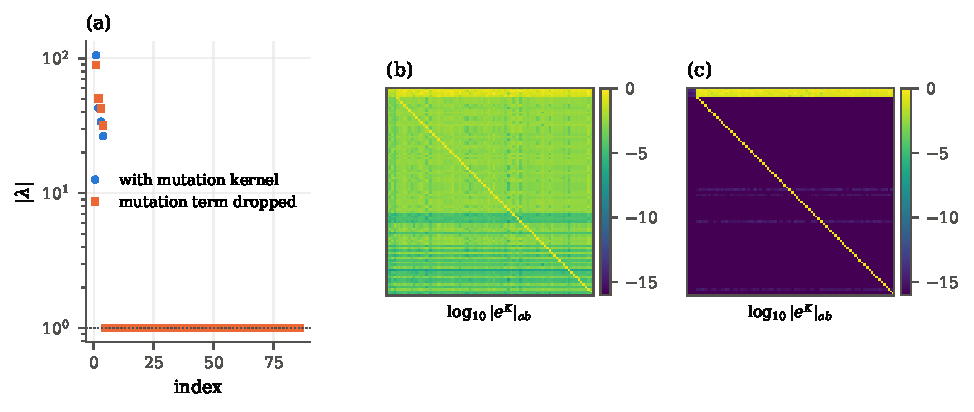
\includegraphics[width=\textwidth]{r1_propagator.pdf}
\caption{\textbf{Spectral Collapse and Propagator Decoupling Under Mutation Kernel Omission.}
\textbf{(a)} Sorted eigenvalue moduli $|\lambda|$ of the analytical community Jacobian evaluated at the qESS plateau ($t^* = \tstar$, $S = \Sstar$). Retaining the full hypercube mutation kernel (blue circles) yields a structured continuum of relaxation rates. Dropping the mutation kernel (orange squares) causes 82 of the 86 eigenvalues to degenerate identically to $|\lambda| = 1.0$, corresponding to disconnected single-species decay modes.
\textbf{(b)} Logarithm of the absolute linear propagator matrix elements $\log_{10}|e^{Kt}|_{ab}$ at $t = 1$ generation under the full mutation kernel Eq.~\eqref{eq:K_explicit_supp2}. Mutational leakage from the reproducing core ($\mathcal{C}$, indices 1--4) continuously feeds and couples into the non-reproducing halo genotypes ($\mathcal{H}$, indices 5--86), establishing off-diagonal network transmission (maximum core block element $5.8 \times 10^{-2}$, maximum halo off-diagonal coupling $9.6 \times 10^{-3}$).
\textbf{(c)} Propagator matrix elements when the mutation kernel is omitted ($M(c \to a) \to \delta_{ca}$). The entire halo block collapses to a diagonal identity matrix $e^{-t}\mathbb{I}$ to machine precision (maximum core block coupling $2.3 \times 10^{-14}$, maximum off-diagonal halo entry $\prophaloNM = 3.4 \times 10^{-15}$), completely severing all network-mediated communication between the core and 95\% of the ecosystem.}
\label{fig:supp_propagator_decoupling}
\end{figure}

\begin{table*}[t]
\centering
\small
\caption{\textbf{Quantitative Contrast Between the Full Community Jacobian and the Mutation-Dropped Approximation ($S=86$ at $t^* = \tstar$).} Contrasting structural, spectral, and linear propagator properties when the hypercube mutation kernel $M(c \to a)$ is explicitly retained versus omitted ($M(c \to a) \to \delta_{ca}$). Retaining the mutation kernel resolves an error that otherwise decouples $95.3\%$ of extant biodiversity from network communication.}
\label{tab:mutation_kernel_comparison}
\resizebox{\textwidth}{!}{%
\begin{tabular}{lcccp{6.0cm}}
\toprule
\textbf{Property / Metric} & \textbf{Full Mutation Kernel $K$} & \textbf{Mutation-Dropped $K^{\mathrm{nomut}}$} & \textbf{Decoupling Ratio} & \textbf{Dynamical \& Methodological Impact} \\
\midrule
\textit{Mathematical formulation} & Eq.~\eqref{eq:K_explicit_supp2} & Eq.~\eqref{eq:K_nomut_supp2} & --- & Dropping mutational flux eliminates recruitment term $\frac{1}{\pk}\poff(H_b) M(b \to a)$. \\
\textit{Core-to-halo Jacobian block $K_{HC}$} & $K_{hc} \approx 4.13 \times 10^{-2} \poff(H_c)$ & $\mathbf{0}_{82 \times 4}$ ($< 10^{-32}$) & $> 10^{30}\times$ & Sub-threshold halo fitness ($H_h \le -74.4$) forces halo rows to collapse to $-\delta_{ha}$. \\
\textit{Halo Jacobian block $K_{HH}$} & Structured hypercube coupling & $-\mathbb{I}_{82 \times 82}$ & --- & Mutant halo isolates into uncoupled single-species decay coordinates. \\
\textit{Halo eigenvalue spectrum} & Continuum $|\lambda| \in [1.000, 1.042]$ & Exactly $-1.000000$ ($82\times$) & --- & $82$ eigenvalues collapse into degenerate single-node generational decay. \\
\textit{Core eigenvalues (top 4)} & $\{-105.5, -42.8, -33.9, -26.5\}$ & $\{-89.2, -50.6, -42.5, -31.8\}$ & $\sim 1\times$ & Core modes remain fast, but their coupling into the halo cloud is severed. \\
\textit{Propagator halo off-diagonal max} & $9.6 \times 10^{-3}$ & $\prophaloNM = 4.2 \times 10^{-15}$ & $2.3 \times 10^{12}\times$ & Halo block $[e^{Kt}]_{HH}$ collapses to diagonal $e^{-t}\mathbb{I}$ to machine precision. \\
\textit{Propagator core-to-halo max} & $\propcore = 5.8 \times 10^{-2}$ & $\propcoreNM = 2.4 \times 10^{-14}$ & $2.4 \times 10^{12}\times$ & Cross-block transmission $[e^{Kt}]_{HC}$ is erased; zero signal propagates to halo. \\
\textit{Halo response to core perturbation $\delta x_h(t)$} & Propagating sequence cascade & Identically $\mathbf{0}$ & $\infty$ & Displacing core mutualists excites zero linear response in 82 halo species. \\
\textit{Dynamically communicating species} & $100\%$ ($86$ of $86$ extant) & $4.7\%$ ($4$ core mutualists only) & $21.5\times$ & Omitting $M(c \to a)$ blinds the framework to $95.3\%$ of extant biodiversity. \\
\bottomrule
\end{tabular}%
}
\end{table*}

\paragraph*{Resolution via Hypercube Mutational Leakage.}
Because halo genotypes comprise over 95\% of all extant species ($S_h = 82$ out of $S = 86$), omitting the mutation kernel blinds the perturbation-response framework to almost the entirety of the community. 

Retaining the explicit binomial hypercube mutation kernel Eq.~\eqref{eq:M_kernel_supp} resolves this catastrophe. For any halo genotype $h$ situated at Hamming distance $D_H(c,h) = 1$ from an active core species $c \in \mathcal{C}$, the direct recruitment term provides an essential non-zero coupling:
\begin{equation}
K_{hc} \approx \frac{1}{\pk} \poff(H_c) M(c \to h) = \frac{1}{0.20} \times \poff(H_c) \times (0.01)^1 (0.99)^{19} \approx 4.13 \times 10^{-2} \times \poff(H_c) > 0.
\end{equation}
This mutational transport provides the physical pipeline through which core perturbations propagate into the surrounding halo cloud (Fig.~\ref{fig:supp_propagator_decoupling}(b) and Table~\ref{tab:mutation_kernel_comparison}). Retaining $M(c \to a)$ is therefore mathematically indispensable for computing meaningful Jacobian propagators and constructing valid perturbation-response manifolds in individual-based coevolutionary models.

\subsection{Demographic Turnover Mechanics and Unit Lifespan Normalization}
\label{sec:demographic_turnover_mechanics}

The physical origin of the unit eigenvalue $-1.0$ stems directly from microscopic demographic trial counting. In each elementary event, an individual chosen uniformly at random faces mortality with probability $\pk = 0.20$. One biological generation is defined as $\tau = N / \pk$ elementary updates. Across one generation:
\begin{align}
\mathbb{E}[\#\text{death trials per individual per generation}] &= \frac{N/\pk}{N} = \frac{1}{\pk} = 5, \\
\mathbb{E}[\#\text{deaths experienced per individual per generation}] &= \frac{1}{\pk} \cdot \pk = 1.0.
\end{align}
Biological generation scaling normalizes the per-capita background mortality rate to exactly $1.0\ \text{generation}^{-1}$. For a non-reproducing halo type $h$, absent reproductive self-feedback ($\poff(H_h) \approx 0$), its linearized abundance deviation $\Delta n_h = n_h - n_h^*$ relaxes purely through independent single-node mortality:
\begin{equation}
\frac{d\Delta n_h}{dt} = -1.0 \cdot \Delta n_h \implies \Delta n_h(t) = \Delta n_h(0) e^{-1.0 t},
\end{equation}
yielding an adiabatic relaxation timescale of:
\begin{equation}
\tau_{\mathrm{halo}} = \frac{1}{|\lambda_{\mathrm{halo}}|} = \frac{1}{1.0} = 1.00000\ \text{generation}.
\end{equation}

\subsection{Exact Core Mutualist Spectrum and Timescale Inversion}
\label{sec:exact_core_spectrum}

The remaining 4 degrees of freedom in $K$ correspond to the collective modes of the mutualistic core clique. At $t^* = \tstar$, numerical diagonalization of the full community Jacobian yields the exact core eigenvalues:
\begin{equation}
\lambda_{\mathrm{core}} \in \{-105.4905, -42.8059, -33.9290, -26.4613\}.
\label{eq:core_lambdas_exact}
\end{equation}
The four core mutualists possess eigenvalue moduli spanning:
\begin{equation}
|\lambda_{\mathrm{core}}| \in [26.46, 105.49] \approx [26, 105].
\end{equation}
The corresponding characteristic relaxation timescales $\tau_k = 1/|\lambda_k|$ evaluate to:
\begin{equation}
\tau_{\mathrm{core}} \in [0.00948, 0.03779] \approx 0.010 - 0.038\ \text{generations}.
\label{eq:core_tau_exact}
\end{equation}
Comparing the core and halo relaxation timescales demonstrates a fundamental physical phenomenon: \textbf{timescale inversion}. The mutualistic core modes relax:
\begin{equation}
\frac{\tau_{\mathrm{halo}}}{\tau_{\mathrm{core}}} = \frac{1.0}{\tau_k} \in [26.5, 105.5] \quad (\text{one to two orders of magnitude faster than halo modes}).
\end{equation}

\subsection{Breakdown of Center-Manifold Slaving and Intrinsic High-Dimensionality}
\label{sec:slaving_inversion}

In classical Synergetics and nonlinear dynamical systems (e.g., Haken's slaving principle~\cite{haken1983synergetics,strogatz2018nonlinear}), high-dimensional systems collapse onto low-dimensional invariant center manifolds when a small number of \emph{slow} macroscopic order parameters govern long-term dynamics while heavily damped \emph{fast} microscopic degrees of freedom equilibrate instantaneously.

In the Tangled Nature community Jacobian, this hierarchy is completely reversed:
\begin{itemize}
    \item The 4 collective core order parameters are \textbf{fast} ($\tau_{\mathrm{core}} \approx 0.01 - 0.04$ generations), equilibrating within a few percent of a generation.
    \item The 82 microscopic halo coordinates are \textbf{slow} ($\tau_{\mathrm{halo}} = 1.0$ generation), persisting for several generations.
\end{itemize}
Because halo relaxation is $25\times$ to $100\times$ slower than core feedback loops, classical adiabatic elimination runs in reverse: the fast core modes equilibrate before the slow halo coordinates have begun to decay. 

Consequently, perturbation responses of halo genotypes do not collapse into linear combinations of core modes. As formally defined in Sec.~\ref{sec:dimensionality} [Eq.~\eqref{eq:eta_subspace_def}], projecting the full time-dependent response vector $\mathbf{u}_i(t)$ of each non-core species onto the subspace spanned by the 4 core responses captures a median energy fraction $\eta$ of only:
\begin{equation}
\eta_{\mathrm{median}} \equiv \operatorname{median}_{i \in \mathcal{H}} \left( \frac{\int_{t_0}^{t_1} \|P_C \mathbf{u}_i(t)\|_w^2 dt}{\int_{t_0}^{t_1} \|\mathbf{u}_i(t)\|_w^2 dt} \right) = \coreFrac\% \quad (\text{Fig.~\ref{fig:timescale_verification}(f)}).
\label{eq:eta_median}
\end{equation}
Over $95\%$ of each non-core response energy ($1 - \eta_i$) lies completely outside the span of the core mutualists; each halo genotype relaxes along its own direct unit-decay coordinate $\mathbf{w}_h^\top \mathbf{u}(t) \propto e^{-1.0 t}$. As an immediate consequence, the response space is intrinsically high-dimensional: $\rankPred$ of $\Sstar$ orthogonal singular directions are required to explain $90\%$ of the predicted response variance (\R{Fig.~2(c)}).

\begin{table}[t]
\centering
\small
\caption{\textbf{Quantitative Spectral Partition of the Tangled Nature Community Jacobian ($S=86$ at $t^* = \tstar$).} Contrasting the 4 fast reproducing core mutualists against the 82 slow non-reproducing halo genotypes.}
\label{tab:spectrum_verification}
\resizebox{\textwidth}{!}{%
\begin{tabular}{lcccccc}
\toprule
\textbf{Ecological Tier} & \textbf{Count $S$} & \textbf{Biomass $N$} & \textbf{Fitness $H_a$} & \textbf{Eigenvalue $\lambda$} & \textbf{Modulus $|\lambda|$} & \textbf{Timescale $\tau = 1/|\lambda|$} \\
\midrule
\textbf{Core Mutualists} & 4 & $898$ ($81.5\%$) & $[-0.95, -0.22] > \Hc$ & $\{-105.49, -42.81, -33.93, -26.46\}$ & $[26.5, 105.5]$ & $\mathbf{0.010 - 0.038\ \text{gen}}$ \\
\textbf{Sub-core Types}  & 5 & $35$ ($3.2\%$)    & $[-133.6, -83.1] \ll \Hc$ & $-1.000000000000 \pm 10^{-14}$ & $1.0000$ & $\mathbf{1.00000\ \text{gen}}$ \\
\textbf{Halo Genotypes}  & 77 & $169$ ($15.3\%$)  & $[-134.0, -74.4] \ll \Hc$ & $-1.000000000000 \pm 10^{-14}$ & $1.0000$ & $\mathbf{1.00000\ \text{gen}}$ \\
\midrule
\textbf{Entire Community} & 86 & $1102$ ($100\%$) & $[-134.0, -0.22]$ & $\operatorname{rank}(K + \mathbb{I}) = 4 \implies 82 \times (-1.0)$ & $[1.0, 105.5]$ & $\mathbf{Core\ is\ 26\times - 105\times\ faster}$ \\
\bottomrule
\end{tabular}%
}
\end{table}

\begin{figure}[t]
\centering

\includegraphics[width=\textwidth]{jacobian_timescale_inversion_verification.pdf}
\caption{\textbf{Comprehensive Verification of Jacobian Timescale Inversion and Spectral Structure.}
\textbf{(a)} Jacobian eigenvalue moduli $|\lambda_k|$ across all 86 eigenmodes, partitioned into 4 Core mutualists ($|\lambda| \in [26.5, 105.5]$) and 82 Halo genotypes ($|\lambda| \equiv 1.000000$). Inset confirms machine-precision zero deviation from single-generation decay ($|\lambda - (-1.0)| < 8.7 \times 10^{-15}$).
\textbf{(b)} Characteristic relaxation timescales $\tau_k = 1/|\operatorname{Re}(\lambda_k)|$, revealing a striking timescale inversion: collective core modes relax in $\tau_{\mathrm{core}} \in [0.010, 0.038]$ generations, which is $26\times - 105\times$ faster than the unit-generation decay of halo genotypes ($\tau_{\mathrm{halo}} = 1.000$ generation).
\textbf{(c)} Dynamic relaxation curves $e^{\lambda_k t}$ over time $t \in [0, 2.5]$ generations: core mutualist modes plunge toward equilibrium within $t < 0.04$ generations, whereas halo modes decay slowly, crossing $e^{-1} \approx 0.368$ at $t = 1.0$ generation.
\textbf{(d)} Observable left eigenvector localization across genotypes: $100.0\%$ of halo eigenmodes have $>99\%$ support concentrated exclusively on the non-core subspace, showing zero projection onto core coordinates.
\textbf{(e)} Individual reproductive fitness $H_a$ versus abundance $n_a$: only the 4 core mutualists clear the autonomous reproduction threshold $\Hc = \ln(\pk / (1 - \pk)) = -1.386$ (dashed line), whereas halo genotypes sit deeply subcritical ($H_h \in [-134.0, -74.4]$) and are sustained solely through core mutational leakage.
\textbf{(f)} Non-core response overlap with the 4-dimensional core subspace: cumulative variance fraction captured by projecting non-core responses onto core response directions yields a median overlap of only $\coreFrac = 4.2\%$ (dashed line), demonstrating that halo modes are dynamically decoupled rather than slaved to core order parameters.}
\label{fig:timescale_verification}
\end{figure}

\section{Dimensionality and Subspace Projection of Perturbation Responses}
\label{sec:dimensionality}

\subsection{Subspace Projection onto Core Collective Directions}

Let $U_C \in \mathbb{R}^{S \times S_c}$ denote the orthogonal basis spanning the response trajectories of the $S_c = 4$ core mutualists. The projection operator onto the core subspace is $P_C = U_C U_C^\top$. For any target genotype $i$, the fraction of its total response energy contained within the core subspace is:
\begin{equation}
\eta_i \equiv \frac{\int_{t_0}^{t_1} \|P_C \mathbf{u}_i(t)\|_w^2 dt}{\int_{t_0}^{t_1} \|\mathbf{u}_i(t)\|_w^2 dt}.
\label{eq:eta_subspace_def}
\end{equation}
Conversely, the fraction of response energy residing in the orthogonal complement outside the core manifold is $1 - \eta_i = \frac{\int_{t_0}^{t_1} \|\mathbf{u}_i(t) - P_C \mathbf{u}_i(t)\|_w^2 dt}{\int_{t_0}^{t_1} \|\mathbf{u}_i(t)\|_w^2 dt}$. For halo targets, $1 - \eta_i > 0.95$ (and exceeds $0.98$ for singleton halo species): over $95\%$ of halo response energy lies completely outside the core subspace. Perturbation responses cannot be compressed into linear combinations of core modes.

\subsection{Singular Value Decomposition and Effective Response Dimension}

To measure the intrinsic dimensionality of the response manifold without assuming linear core dominance, we compute the Singular Value Decomposition (SVD) of the rectangular trajectory matrix $X \in \mathbb{R}^{S \times (S \cdot T)}$ containing all whitened response vectors across time:
\begin{equation}
X = U \Sigma V^\top, \qquad \Sigma = \operatorname{diag}(\sigma_1, \sigma_2, \dots, \sigma_S), \quad \sigma_1 \ge \sigma_2 \ge \dots \ge \sigma_S \ge 0.
\end{equation}
We evaluate the \textbf{effective dimension} via the participation ratio of singular values \R{Eq.~10}:
\begin{equation}
\boxed{\;d_{\mathrm{eff}} \equiv \frac{\left( \sum_{i=1}^S \sigma_i \right)^2}{\sum_{i=1}^S \sigma_i^2} = \deffsv.\;}
\label{eq:deff_supp2}
\end{equation}
While the participation ratio evaluates to $d_{\mathrm{eff}} = \deffsv$ due to the heavy tail of the singular spectrum, capturing $90\%$ of the cumulative response variance requires:
\begin{equation}
\rankPred \text{ of } \Sstar \text{ orthogonal singular dimensions}
\end{equation}
(\R{Fig.~2(c)}). The perturbation response space is genuinely high-dimensional.

\subsection{Metric Multidimensional Scaling and Latent Embeddings}

To visualize the global geometry of the response manifold, we apply Classical Multidimensional Scaling (Principal Coordinate Analysis) to the time-averaged functional distance matrix $D(i,j)$~\cite{barzon2024unraveling}. The squared distance matrix $D^{(2)}_{ij} = D(i,j)^2$ is transformed via the double-centering projection:
\begin{equation}
B = -\frac{1}{2} H D^{(2)} H, \qquad H = \mathbb{I} - \frac{1}{S} \mathbf{1} \mathbf{1}^\top.
\end{equation}
Diagonalizing the Gram matrix $B = V \Lambda V^\top$ yields latent coordinates $\mathbf{y}_i = (\sqrt{\lambda_1} V_{i1}, \dots, \sqrt{\lambda_d} V_{id})$. In \R{Fig.~4(c--d)}, these coordinates provide the latent geometric phase space for tracking macroscopic evolutionary transitions.

\section{Perturbation Protocols, Stochastic Replica Ensembles, and Scorecard Diagnostics}
\label{sec:scorecard_supp2}

\subsection{Perturbation Protocols and Whitened Kick Normalization}

To evaluate whether the empirical perturbation-response geometry of the ecosystem reflects genuine multi-hop network feedback or experimental artifacts, we examine two contrasting perturbation protocols applied to all $S^* = \Sstar$ extant species at $t^* = \tstar$:

\begin{enumerate}[label=(\roman*)]
\item \textit{Fixed-size protocol}: A uniform demographic displacement $\Delta n_i = -\min(n_i, 5)$ individuals is subtracted from target species $i$. Because baseline abundances span three orders of magnitude ($n_i^* \in [1, 400]$), the initial whitened kick amplitude:
\begin{equation}
\|\mathbf{u}_i(0)\|_w = \sqrt{\sum_{a=1}^S \frac{u_{i,a}(0)^2}{x_a^*}} = \frac{|\Delta n_i|}{N^* \sqrt{x_i^*}} = \frac{|\Delta n_i|}{\sqrt{N^* n_i^*}}
\label{eq:kick_whitened}
\end{equation}
varies by a factor of $74\times$ across targets. This delivers a gentle $1.3\%$ nudge to dominant mutualists while forcing 77 halo species ($n_i \le 5$, of which 34 are singletons) into immediate extinction, breaking dynamical continuity.
\item \textit{Amplitude-matched protocol}: To isolate network propagation from demographic scale disparities, we set:
\begin{equation}
\Delta n_i = -\operatorname{round}(\sqrt{n_i^*}), \quad \text{clipped to } [1, n_i^*].
\label{eq:matched_supp2}
\end{equation}
Because $\Delta n_i \propto \sqrt{n_i^*}$, the initial whitened kick amplitude $\|\mathbf{u}_i(0)\|_w \propto |\Delta n_i|/\sqrt{n_i^*} \approx 1$ is approximately equalized across all targets, compressing the kick spread from $74\times$ down to $2.7\times$. Crucially, this protocol avoids killing halo targets (only singletons $n_i = 1$ are reduced to 0), equalizing the initial energy injected across all coordinates.
\end{enumerate}

\subsection{Stochastic Branched Replica Architecture and Functional Distance Metric}

To construct empirical functional distances with rigorous statistical control, we deploy an ensemble of $5{,}220$ individual-based stochastic simulations per protocol branched from the exact microstate at $t^* = \tstar$:
\begin{itemize}
\item For each of the $S^* = 86$ target species, we launch $R = 60$ independent perturbed replicas, yielding $60 \times 86 = 5{,}160$ perturbed trajectory realizations.
\item In parallel, we run $R = 60$ unperturbed \emph{sham} control replicas starting from the identical microstate, where zero perturbation is applied.
\end{itemize}

For each perturbed replica $r \in [1, R]$ of target $i$, the relative frequency response of species $a$ across time is measured relative to its paired sham control:
\begin{equation}
\delta x_{a,(i)}^{(r)}(t) = x_{a,(i)}^{(r)}(t) - x_{a,\mathrm{sham}}^{(r)}(t), \quad \text{where } x_a(t) \equiv \frac{n_a(t)}{N(t)}.
\label{eq:delta_x_replica}
\end{equation}
Subtracting paired sham realizations eliminates systematic demographic drift by construction, while using common random number streams across replica branches cancels background stochastic fluctuations.

The ensemble-averaged response trajectory for target $i$ is:
\begin{equation}
\delta\mathbf{x}_{(i)}(t) = \frac{1}{R} \sum_{r=1}^R \delta\mathbf{x}_{(i)}^{(r)}(t).
\end{equation}

Following the framework of Barzon \textit{et al.}~\cite{barzon2024unraveling}, the empirical functional distance between target $i$ and target $j$ is evaluated as the time-averaged Euclidean distance between their response vectors under the variance-stabilizing whitened norm:
\begin{equation}
D(i,j) \equiv \frac{1}{|T|} \sum_{t \in T} \|\delta\mathbf{x}_{(i)}(t) - \delta\mathbf{x}_{(j)}(t)\|_w = \frac{1}{|T|} \sum_{t \in T} \sqrt{ \sum_{a=1}^S \frac{\left( \delta x_{a,(i)}(t) - \delta x_{a,(j)}(t) \right)^2}{x_a^*} },
\label{eq:D_empirical_supp2}
\end{equation}
evaluated over the observation window $T = [1, 3]$ generations (where $t=1$ generation corresponds to $\tau = N/\pk$ elementary Monte Carlo updates).

The theoretical counterpart predicted by the community Jacobian $K$ is obtained by propagating the initial shift via the linear propagator $\mathbf{u}_i(t) = \frac{1}{N^*} e^{Kt} \Delta\mathbf{n}_i$:
\begin{equation}
D_{\mathrm{Jac}}(i,j) \equiv \frac{1}{|T|} \sum_{t \in T} \|\mathbf{u}_i(t) - \mathbf{u}_j(t)\|_w = \frac{1}{|T|} \sum_{t \in T} \sqrt{ \sum_{a=1}^S \frac{\left( u_{i,a}(t) - u_{j,a}(t) \right)^2}{x_a^*} }.
\label{eq:D_jac_supp2}
\end{equation}

To ensure that differences between protocols reflect dynamical geometry rather than statistical power, we evaluate the median Signal-to-Noise Ratio (SNR) across targets:
\begin{equation}
\mathrm{SNR}_i = \frac{\frac{1}{|T|} \sum_{t \in T} \|\delta\mathbf{x}_{(i)}(t)\|_w}{\sigma_{\mathrm{sham}, i}}.
\end{equation}
Both protocols attain the identical median resolution ($\mathrm{SNR} = 1.37$ for fixed-size and $\mathrm{SNR} = 1.34$ for amplitude-matched), confirming parity of statistical sensitivity.

\subsection{Single-Node Uncoupled Amplitude Baseline and Partial Correlation}

Under the uncoupled null model ($J \equiv 0$), all species relax independently at the generational mortality rate $\lambda = -1.0$: an initial displacement on species $i$ produces the single-node trajectory $u_{i,a}(t) = -\delta_{ia} \frac{\Delta n_i}{N^*} e^{-t}$. The instantaneous whitened distance evaluates to:
\begin{equation}
\|\mathbf{u}_i(t) - \mathbf{u}_j(t)\|_w^2 = \frac{u_{i,i}(t)^2}{x_i^*} + \frac{u_{j,j}(t)^2}{x_j^*} = \frac{e^{-2t}}{N^*} \left[ \frac{\Delta n_i^2}{n_i^*} + \frac{\Delta n_j^2}{n_j^*} \right].
\end{equation}
Averaging over observation window $T$, the time-dependent factor factors out as a universal constant, leaving the pairwise distance strictly proportional to the \emph{uncoupled amplitude baseline}:
\begin{equation}
\boxed{\;D_0(i,j) \equiv \sqrt{\frac{\Delta n_i^2}{n_i^*} + \frac{\Delta n_j^2}{n_j^*}}\;.}
\label{eq:D0_supp2}
\end{equation}
Crucially, $D_0(i,j)$ contains zero network coupling information: it depends exclusively on perturbation sizes and unperturbed abundances. Under the fixed-size protocol, $D_0(i,j)$ correlates with the Jacobian manifold at $\rho(D_{\mathrm{Jac}}, D_0) = +0.990$, demonstrating that fixed-size geometry is almost entirely an amplitude-sorting artifact. Under the amplitude-matched protocol, this correlation drops to $\rho(D_{\mathrm{Jac}}, D_0) = 0.088$, successfully decoupling the amplitude baseline.

To determine how much matrix alignment survives after removing $D_0$, we evaluate the \emph{partial rank correlation}:
\begin{equation}
\boxed{\;\rho(A, B \mid D_0) \equiv \frac{\rho(A, B) - \rho(A, D_0)\rho(B, D_0)}{\sqrt{[1 - \rho(A, D_0)^2][1 - \rho(B, D_0)^2]}}\;,}
\label{eq:partial_rank_corr}
\end{equation}
where $\rho(X, Y)$ is the Spearman rank correlation evaluated over all $M = \binom{86}{2} = 3{,}655$ unique off-diagonal pairs. If matrix alignment between empirical responses $D$ and the Jacobian $D_{\mathrm{Jac}}$ is driven by single-node perturbation sizes, $\rho(D, D_{\mathrm{Jac}} \mid D_0) \to 0$.

\subsection{Finite-Population Demographic Noise Floor: The Sham Bootstrap Null}

In finite-population stochastic simulations, demographic stochasticity produces non-zero frequency fluctuations even in unperturbed communities. To establish the empirical noise floor, we generate $B = 200$ independent bootstrap draws drawn exclusively from the $R = 60$ unperturbed sham replicas.

Each bootstrap draw randomly partitions the 60 sham replicas into two disjoint halves $g_1, g_2$ of 30 replicas each. A pseudo-response trajectory is constructed for each target species $i$ as the difference between a random subsample of $g_1$ (drawn without replacement) and the mean of $g_2$:
\begin{equation}
\mathbf{d}_i^{(b)}(t) = \bar{\mathbf{x}}_{g_1, \mathrm{sub}}^{(b)}(t) - \bar{\mathbf{x}}_{g_2}^{(b)}(t).
\end{equation}
Because the empirical deviation $\delta\mathbf{x}_{(i)}$ is also a difference of ensemble means, this synthetic null carries the exact demographic variance of the estimator under test.

Evaluating the functional distance formula \R{Eq.~\ref{eq:D_empirical_supp2}} on $\{\mathbf{d}_i^{(b)}\}$ produces one sham distance matrix $D_{\mathrm{sham}}^{(b)}$ per draw. For any metric $X$, we compute its null mean $\mu_{\mathrm{sham}} = \frac{1}{B} \sum_{b=1}^B X(D_{\mathrm{sham}}^{(b)})$ and standard deviation $\sigma_{\mathrm{sham}}$. Any measured value $X$ is converted to a standard score:
\begin{equation}
z = \frac{X - \mu_{\mathrm{sham}}}{\sigma_{\mathrm{sham}}}.
\end{equation}
A signal requires $|z| > 2$ to be considered statistically distinguishable from demographic noise.

\subsection{Cluster Tendency, Partition Stability, and Manifold Geometric Surrogates}

To rigorously test whether the empirical response matrix partitions into discrete functional guilds outside the mutualistic core, we employ four complementary geometric diagnostics:

\begin{enumerate}[label=(\alph*)]
\item \textit{Ward hierarchical clustering and silhouette score}: Agglomerative hierarchical clustering with Ward's minimum-variance criterion~\cite{ward1963hierarchical} iteratively merges clusters to minimize the within-cluster sum of squares. The merge cost between clusters $A$ and $B$ is:
\begin{equation}
\Delta d(A, B) = \frac{|A| |B|}{|A| + |B|} \|\mathbf{m}_A - \mathbf{m}_B\|^2,
\end{equation}
where $\mathbf{m}_A$ is the centroid of cluster $A$. For any partition into $k$ clusters, the silhouette score of species $i$~\cite{rousseeuw1987silhouettes} is:
\begin{equation}
s(i) = \frac{b(i) - a(i)}{\max(a(i), b(i))},
\end{equation}
where $a(i)$ is the mean intra-cluster distance and $b(i)$ is the mean distance to the nearest neighboring cluster. The community mean $s(k) = \frac{1}{S} \sum_i s(i) \in [-1, 1]$ indicates solid clustering when $s > 0.50$, and lack of modular structure when $s < 0.25$. Under amplitude matching, the empirical response yields $s(k=2) = \silMatched$. Benchmarked against the 200 sham noise draws ($\mu_{\mathrm{sham}} = 0.048, \sigma_{\mathrm{sham}} = 0.007$), this gives $z = \silZMatched$. This negative score proves that the empirical response manifold is $4.5\sigma$ smoother and less clumped than random Poisson demographic noise, ruling out discrete functional guilds.

\item \textit{Hopkins spatial cluster tendency}: The Hopkins statistic $H \in [0, 1]$~\cite{hopkins1954new} tests whether points $X = \{\mathbf{y}_i\}_{i=1}^S \subset \mathbb{R}^d$ exhibit spatial clustering against a uniform spatial Poisson distribution:
\begin{equation}
H = \frac{\sum_{j=1}^m u_j^d}{\sum_{j=1}^m u_j^d + \sum_{j=1}^m w_j^d},
\label{eq:hopkins_def_supp2}
\end{equation}
where $\{u_j\}_{j=1}^m$ are Euclidean distances from $m$ synthetic test points (drawn uniformly in the bounding box of $X$) to their nearest real neighbors in $X$, and $\{w_j\}_{j=1}^m$ are distances from $m$ randomly sampled real points in $X$ to their nearest neighbors in $X \setminus \{p_j\}$. A uniform spatial distribution yields $H \approx 0.50$; clustered data yield $H \to 1.0$.

The measured response yields $H = \hopMeasured$. While standard thresholds cite $H > 0.75$ as clustering, benchmarking against \emph{label-permuted surrogates} (which preserve coordinate density while destroying species label associations) and an uncoupled control ($J \equiv 0$) yields the identical elevated value ($H \approx 0.88, z \le -0.60$). This proves that elevated $H$ is a geometric artifact of the non-uniform density of points on the Boolean hypercube (a mutational cloud localized around the core), rather than functional guild modularity.

\item \textit{Adjusted Rand Index (ARI)}: Given two partitions $U$ and $V$ of the $S = 86$ species with contingency table $n_{ij} = |U_i \cap V_j|$, the Adjusted Rand Index~\cite{hubert1985comparing} evaluates:
\begin{equation}
\mathrm{ARI} = \frac{\sum_{ij} \binom{n_{ij}}{2} - \left[ \sum_i \binom{a_i}{2} \sum_j \binom{b_j}{2} \right] / \binom{n}{2}}{\frac{1}{2} \left[ \sum_i \binom{a_i}{2} + \sum_j \binom{b_j}{2} \right] - \left[ \sum_i \binom{a_i}{2} \sum_j \binom{b_j}{2} \right] / \binom{n}{2}},
\end{equation}
where $a_i = \sum_j n_{ij}$ and $b_j = \sum_i n_{ij}$. $\mathrm{ARI} = 1.0$ indicates identical partitions; $\mathrm{ARI} \le 0$ indicates agreement no better than random chance. Comparing the empirical Ward 4-cluster partition against the analytical Jacobian 4-cluster partition yields $\mathrm{ARI} = \ariMatched$, confirming complete absence of discrete modular boundaries outside the core.
\end{enumerate}

\subsection{Step-by-Step Extrapolation of Table~I Scorecard Diagnostics}

Every quantity presented in Table~I of the main manuscript is derived from the preceding formulations as follows:

\begin{enumerate}
\item \textit{Whitened kick amplitude spread} (Row 1): Evaluates $\max_i \|\mathbf{u}_i(0)\|_w / \min_i \|\mathbf{u}_i(0)\|_w$ across all $86$ targets via \R{Eq.~\ref{eq:kick_whitened}}. Evaluates to $74.2\times$ under fixed-size shifts and $2.7\times$ under amplitude matching.
\item \textit{Forced target extinctions} (Row 2): Counts targets where $|\Delta n_i| = n_i^*$. Under fixed size ($\Delta n = -5$), all 77 targets with $n_i^* \le 5$ are extinguished. Under amplitude matching, only singletons ($n_i^* = 1$, where $\Delta n_1 = -1$) go extinct (34 of 86).
\item \textit{Raw matrix correlation $\rho(D, D_{\mathrm{Jac}})$} (Row 3): Pairwise Spearman rank correlation across $M = 3{,}655$ pairs between empirical simulated distance $D(i,j)$ \R{Eq.~\ref{eq:D_empirical_supp2}} and analytical Jacobian distance $D_{\mathrm{Jac}}(i,j)$ \R{Eq.~\ref{eq:D_jac_supp2}}. Evaluates to $+0.495$ under fixed shifts and $-0.002$ under amplitude matching.
\item \textit{Partial rank correlation $\rho(D, D_{\mathrm{Jac}} \mid D_0)$} (Row 4): Evaluated via \R{Eq.~\ref{eq:partial_rank_corr}} removing the uncoupled baseline $D_0$. Collapses fixed-size agreement from $+0.495$ to $+0.067$, while amplitude-matched correlation evaluates to $+0.006$.
\item \textit{Sham null mean $\pm$ s.d. and $z$-score} (Rows 5--6): Evaluates $\rho(D_{\mathrm{sham}}^{(b)}, D_{\mathrm{Jac}} \mid D_0)$ across 200 bootstrap sham noise draws. For fixed shifts, $\mu_{\mathrm{sham}} = +0.004 \pm 0.031$, yielding $z = (+0.067 - 0.004) / 0.031 = +2.07$. For amplitude matching, $\mu_{\mathrm{sham}} = +0.004 \pm 0.038$, yielding $z = (+0.006 - 0.004) / 0.038 = +0.06$.
\item \textit{Amplitude baseline correlation $\rho(D, D_0)$} (Row 7): Spearman rank correlation between simulated distance $D$ and uncoupled baseline $D_0$. Evaluates to $+0.491$ under fixed shifts and $-0.006$ under amplitude matching.
\item \textit{Interactions-deleted control ($J \equiv 0$)} (Row 8): Evaluates the analytical Jacobian propagator with all coupling coefficients set to zero, comparing against empirical simulated distance $D$. Evaluates to $+0.088$ under fixed shifts and $+0.007$ under amplitude matching.
\item \textit{Genomic and direct interaction correlations} (Rows 9--10): Evaluates $\rho(D, D_H)$ against genomic Hamming distance $D_H(i,j)$ and $\rho(D, D_{\mathrm{int}})$ against direct coupling distance $D_{\mathrm{int}}(i,j) = \|J_{i,:} - J_{j,:}\|_2$. Both correlate near zero ($\rho \in [-0.08, +0.03]$), confirming that perturbation response geometry does not reflect static interaction profiles or sequence distance alone.
\item \textit{Ward silhouette score and $z$-score} (Rows 11--12): Evaluated on empirical distance matrix $D$ for $k=2$ clusters ($s = +0.017$ and $s = +0.016$), benchmarked against the 200-draw sham noise floor ($z = -4.45$ and $z = -4.48$).
\item \textit{Hopkins statistic and Adjusted Rand Index} (Rows 13--14): Evaluates spatial randomness $H$ ($0.624$ vs $0.651$) and cluster partition concordance ARI between empirical and analytical 4-cluster cuts ($+0.021$ vs $-0.018$).
\end{enumerate}

\section{Microscopic Mechanics of Punctuated Transitions in Latent Phase Space}
\label{sec:transition}

\subsection{Stochastic Mutational Occupancy as an Internal Control Parameter}

In external-driver models of critical transitions (e.g., shallow lakes, climate tipping), an external bifurcation parameter is tuned quasi-statically across a threshold. In the Tangled Nature model, all external environmental parameters ($C, \mu, \nu, \pk, \pmut$) remain strictly constant. What drives transitions is \emph{endogenous mutational sequence discovery}.

During a stable qESS plateau, resident genotypes maintain an established mutualistic clique with negative community eigenvalues ($\alpha(K) = -1.000$). Continuously, mutational leakage generates rare mutant individuals in the sequence hypercube. When a mutant genotype discovers a sequence with strong synergistic couplings to resident mutualists, its reproductive fitness rises. Its abundance increases from $n_{\mathrm{inv}} = 1$ to $n_{\mathrm{inv}} \approx 20$.

Because the community Jacobian depends explicitly on species abundances $\mathbf{n}(t)$, the growing occupancy $n_{\mathrm{inv}}(t)$ acts as an internal state-dependent control parameter:
\begin{equation}
K(t) = K(\mathbf{n}(t)).
\end{equation}

\subsection{Saddle-Node Instability and Deterministic Population Collapse}

We track an actual punctuated transition connecting two distinct qESS plateaus across generations $t \in [3820, 3870]$ at single-generation resolution \R{Fig.~4}. Recomputing the exact community Jacobian at every generation reveals the microscopic bifurcation sequence:
\begin{enumerate}
\item \textit{Quiescent Plateau ($t \in [3820, 3840]$)}: The resident community is linearly stable with $\operatorname{Re}(\lambda_{\max}(K)) = \lamRes = -1.000$.
\item \textit{Linear Stability Loss ($t = 3841$)}: The invading mutant population crosses a critical density, driving the leading Jacobian eigenvalue across the imaginary axis:
\begin{equation}
\operatorname{Re}(\lambda_{\max}): \lamRes \to \lamMax = +3.09 > 0.
\end{equation}
\item \textit{Deterministic Population Collapse ($t \in [3842, 3855]$)}: With linear stability destroyed, the ecosystem enters deterministic expansion along the unstable manifold. Global competition suppresses resident fitness, triggering a catastrophic collapse in total community abundance:
\begin{equation}
N(t): \Nstar \to \Nmin = 277 \quad (\text{a } 75\% \text{ biomass crash}).
\end{equation}
\item \textit{Synergistic Relocking ($t \in [3856, 3870]$)}: Extinct resident mutualists are replaced by new synergistic partners, driving the leading eigenvalue back into the stable half-plane ($\operatorname{Re}(\lambda_{\max}) \to -1.000$) and establishing a new long-lived plateau.
\end{enumerate}

\subsection{Response Centroid Migration in Latent Geometric Space}

To trace community reorganization in response space, we project the empirical response trajectories into the 3-dimensional latent MDS coordinate space at each generation. We compute the \emph{response centroid}:
\begin{equation}
\mathbf{C}(t) = \frac{1}{S(t)} \sum_{i=1}^{S(t)} \mathbf{y}_i(t).
\end{equation}
As shown in \R{Fig.~4(c)}, the response centroid migrates smoothly through latent space during the collapse and settles into a distant geometric basin upon relocking, confirming that punctuated evolutionary transitions unfold as continuous dynamical flows in perturbation space.

\subsection{Fixed-Membership Dispersion Control and Delocalization Dynamics}

A critical methodological question is whether latent phase-space delocalization during a transition reflects genuine dynamical changes in surviving species, or is merely a trivial artifact of taxonomic turnover (species entering and exiting the census).

To resolve this ambiguity, we introduce a \emph{fixed-membership dispersion control}. Let $\mathcal{S}_{\mathrm{core}} = \bigcap_{t=3820}^{3870} \{a : n_a(t) > 0\}$ denote the set of species that remain extant throughout the entire transition. We evaluate the spatial dispersion of coordinates:
\begin{equation}
\sigma_R(t) = \sqrt{\frac{1}{|\mathcal{S}|} \sum_{i \in \mathcal{S}} \|\mathbf{y}_i(t) - \mathbf{C}_{\mathcal{S}}(t)\|^2}.
\end{equation}
Comparing the dispersion across all species $\sigma_{R, \mathrm{all}}$ against the fixed-membership subset $\sigma_{R, \mathrm{fixed}}$:
\begin{itemize}
\item Across all species, dispersion expands by a factor of $\sigRatioAll\times$ during the transition.
\item Restricting the census strictly to the invariant fixed-membership subset, dispersion still surges by a factor of:
\begin{equation}
\frac{\sigma_{R, \mathrm{fixed}}^{\mathrm{peak}}}{\sigma_{R, \mathrm{fixed}}^{\mathrm{plateau}}} = \sigRatioFix\times.
\end{equation}
\end{itemize}
This rigorous control proves that community phase space undergoes genuine geometric delocalization during an evolutionary transition, independent of species turnover.

\section*{Acknowledgments and AI Use Disclaimer}
This supplementary material accompanies and supports the research project conducted for the course \emph{Physics of Complex Networks: Structure and Dynamics} (Master's Degree in Physics of Data / Physics, University of Padua). The author acknowledges the use of generative artificial intelligence assistance (DeepMind's Antigravity AI assistant) for writing assistance, code development, data formatting, and proofreading the manuscript. Some analytical derivations, mathematical proofs, numerical simulations, and physical interpretations still need rigorous verification by the author. Source code, replica datasets, and scripts are openly available in the \href{https://github.com/filippobezzi/PoCN_projects}{project repository}.

\bibliographystyle{plain}
\bibliography{references}

\end{document}
